\documentclass[twoside]{book}

% Packages required by doxygen
\usepackage{fixltx2e}
\usepackage{calc}
\usepackage{doxygen}
\usepackage[export]{adjustbox} % also loads graphicx
\usepackage{graphicx}
\usepackage[utf8]{inputenc}
\usepackage{makeidx}
\usepackage{multicol}
\usepackage{multirow}
\PassOptionsToPackage{warn}{textcomp}
\usepackage{textcomp}
\usepackage[nointegrals]{wasysym}
\usepackage[table]{xcolor}

% Font selection
\usepackage[T1]{fontenc}
\usepackage[scaled=.90]{helvet}
\usepackage{courier}
\usepackage{amssymb}
\usepackage{sectsty}
\renewcommand{\familydefault}{\sfdefault}
\allsectionsfont{%
  \fontseries{bc}\selectfont%
  \color{darkgray}%
}
\renewcommand{\DoxyLabelFont}{%
  \fontseries{bc}\selectfont%
  \color{darkgray}%
}
\newcommand{\+}{\discretionary{\mbox{\scriptsize$\hookleftarrow$}}{}{}}

% Page & text layout
\usepackage{geometry}
\geometry{%
  a4paper,%
  top=2.5cm,%
  bottom=2.5cm,%
  left=2.5cm,%
  right=2.5cm%
}
\tolerance=750
\hfuzz=15pt
\hbadness=750
\setlength{\emergencystretch}{15pt}
\setlength{\parindent}{0cm}
\setlength{\parskip}{3ex plus 2ex minus 2ex}
\makeatletter
\renewcommand{\paragraph}{%
  \@startsection{paragraph}{4}{0ex}{-1.0ex}{1.0ex}{%
    \normalfont\normalsize\bfseries\SS@parafont%
  }%
}
\renewcommand{\subparagraph}{%
  \@startsection{subparagraph}{5}{0ex}{-1.0ex}{1.0ex}{%
    \normalfont\normalsize\bfseries\SS@subparafont%
  }%
}
\makeatother

% Headers & footers
\usepackage{fancyhdr}
\pagestyle{fancyplain}
\fancyhead[LE]{\fancyplain{}{\bfseries\thepage}}
\fancyhead[CE]{\fancyplain{}{}}
\fancyhead[RE]{\fancyplain{}{\bfseries\leftmark}}
\fancyhead[LO]{\fancyplain{}{\bfseries\rightmark}}
\fancyhead[CO]{\fancyplain{}{}}
\fancyhead[RO]{\fancyplain{}{\bfseries\thepage}}
\fancyfoot[LE]{\fancyplain{}{}}
\fancyfoot[CE]{\fancyplain{}{}}
\fancyfoot[RE]{\fancyplain{}{\bfseries\scriptsize Generated by Doxygen }}
\fancyfoot[LO]{\fancyplain{}{\bfseries\scriptsize Generated by Doxygen }}
\fancyfoot[CO]{\fancyplain{}{}}
\fancyfoot[RO]{\fancyplain{}{}}
\renewcommand{\footrulewidth}{0.4pt}
\renewcommand{\chaptermark}[1]{%
  \markboth{#1}{}%
}
\renewcommand{\sectionmark}[1]{%
  \markright{\thesection\ #1}%
}

% Indices & bibliography
\usepackage{natbib}
\usepackage[titles]{tocloft}
\setcounter{tocdepth}{3}
\setcounter{secnumdepth}{5}
\makeindex

% Hyperlinks (required, but should be loaded last)
\usepackage{ifpdf}
\ifpdf
  \usepackage[pdftex,pagebackref=true]{hyperref}
\else
  \usepackage[ps2pdf,pagebackref=true]{hyperref}
\fi
\hypersetup{%
  colorlinks=true,%
  linkcolor=blue,%
  citecolor=blue,%
  unicode%
}

% Custom commands
\newcommand{\clearemptydoublepage}{%
  \newpage{\pagestyle{empty}\cleardoublepage}%
}

\usepackage{caption}
\captionsetup{labelsep=space,justification=centering,font={bf},singlelinecheck=off,skip=4pt,position=top}

%===== C O N T E N T S =====

\begin{document}

% Titlepage & ToC
\hypersetup{pageanchor=false,
             bookmarksnumbered=true,
             pdfencoding=unicode
            }
\pagenumbering{alph}
\begin{titlepage}
\vspace*{7cm}
\begin{center}%
{\Large Heisprosjekt }\\
\vspace*{1cm}
{\large Generated by Doxygen 1.8.13}\\
\end{center}
\end{titlepage}
\clearemptydoublepage
\pagenumbering{roman}
\tableofcontents
\clearemptydoublepage
\pagenumbering{arabic}
\hypersetup{pageanchor=true}

%--- Begin generated contents ---
\chapter{File Index}
\section{File List}
Here is a list of all documented files with brief descriptions\+:\begin{DoxyCompactList}
\item\contentsline{section}{source/\hyperlink{buttons__lights__doors_8c}{buttons\+\_\+lights\+\_\+doors.\+c} \\*Implementation of functions for buttons, lights and doors }{\pageref{buttons__lights__doors_8c}}{}
\item\contentsline{section}{source/\hyperlink{buttons__lights__doors_8h}{buttons\+\_\+lights\+\_\+doors.\+h} \\*Functions for buttons, lights and doors }{\pageref{buttons__lights__doors_8h}}{}
\item\contentsline{section}{source/\hyperlink{elevator__logic_8c}{elevator\+\_\+logic.\+c} \\*Implementation of functions to create the elevator logic }{\pageref{elevator__logic_8c}}{}
\item\contentsline{section}{source/\hyperlink{elevator__logic_8h}{elevator\+\_\+logic.\+h} \\*Functions to create the elevator logic }{\pageref{elevator__logic_8h}}{}
\item\contentsline{section}{source/\hyperlink{hardware_8h}{hardware.\+h} \\*Driver for the elevator hardware }{\pageref{hardware_8h}}{}
\item\contentsline{section}{source/\hyperlink{main_8c}{main.\+c} \\*Main file for running the elevator code. while loop handling movement of elevator }{\pageref{main_8c}}{}
\item\contentsline{section}{source/\hyperlink{safety_8c}{safety.\+c} \\*Implementation of safety functions }{\pageref{safety_8c}}{}
\item\contentsline{section}{source/\hyperlink{safety_8h}{safety.\+h} \\*Safety functions for the elevator }{\pageref{safety_8h}}{}
\end{DoxyCompactList}

\chapter{File Documentation}
\hypertarget{button__operations_8c}{}\section{source/button\+\_\+operations.c File Reference}
\label{button__operations_8c}\index{source/button\+\_\+operations.\+c@{source/button\+\_\+operations.\+c}}


implementation of button operation functions  


{\ttfamily \#include $<$stdio.\+h$>$}\newline
{\ttfamily \#include $<$stdlib.\+h$>$}\newline
{\ttfamily \#include \char`\"{}hardware.\+h\char`\"{}}\newline
Include dependency graph for button\+\_\+operations.\+c\+:\nopagebreak
\begin{figure}[H]
\begin{center}
\leavevmode
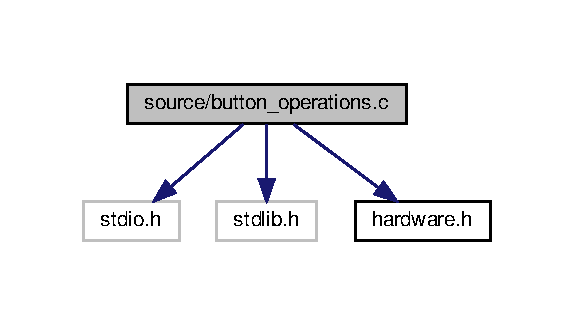
\includegraphics[width=276pt]{button__operations_8c__incl}
\end{center}
\end{figure}
\subsection*{Functions}
\begin{DoxyCompactItemize}
\item 
\mbox{\Hypertarget{button__operations_8c_a1ef434f57c0cde9e2dca0f8d5a9235ab}\label{button__operations_8c_a1ef434f57c0cde9e2dca0f8d5a9235ab}} 
void {\bfseries stop\+\_\+button\+\_\+pushed} (\hyperlink{hardware_8h_a2167c399a24df296afc432bcb88228af}{Hardware\+Movement} current\+\_\+movement)
\item 
\mbox{\Hypertarget{button__operations_8c_a258e3b580e688a0cf46e4258525aeaf1}\label{button__operations_8c_a258e3b580e688a0cf46e4258525aeaf1}} 
void \hyperlink{button__operations_8c_a258e3b580e688a0cf46e4258525aeaf1}{sigint\+\_\+handler} (int sig)
\begin{DoxyCompactList}\small\item\em Stop elevator. \end{DoxyCompactList}\end{DoxyCompactItemize}


\subsection{Detailed Description}
implementation of button operation functions 


\hypertarget{button__operations_8h}{}\section{source/button\+\_\+operations.h File Reference}
\label{button__operations_8h}\index{source/button\+\_\+operations.\+h@{source/button\+\_\+operations.\+h}}


functions for button operations  


This graph shows which files directly or indirectly include this file\+:
\nopagebreak
\begin{figure}[H]
\begin{center}
\leavevmode
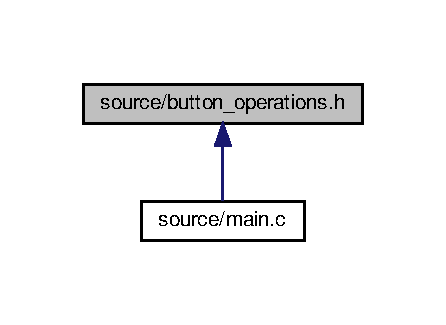
\includegraphics[width=214pt]{button__operations_8h__dep__incl}
\end{center}
\end{figure}
\subsection*{Functions}
\begin{DoxyCompactItemize}
\item 
\mbox{\Hypertarget{button__operations_8h_a10ff64f279bc37be638909f77035ad43}\label{button__operations_8h_a10ff64f279bc37be638909f77035ad43}} 
void \hyperlink{button__operations_8h_a10ff64f279bc37be638909f77035ad43}{stop\+\_\+button\+\_\+pushed} ()
\begin{DoxyCompactList}\small\item\em stop the elevator when button is pushed \end{DoxyCompactList}\item 
\mbox{\Hypertarget{button__operations_8h_a258e3b580e688a0cf46e4258525aeaf1}\label{button__operations_8h_a258e3b580e688a0cf46e4258525aeaf1}} 
void \hyperlink{button__operations_8h_a258e3b580e688a0cf46e4258525aeaf1}{sigint\+\_\+handler} (int sig)
\begin{DoxyCompactList}\small\item\em Stop elevator. \end{DoxyCompactList}\end{DoxyCompactItemize}


\subsection{Detailed Description}
functions for button operations 


\hypertarget{floor__operations_8c}{}\section{source/floor\+\_\+operations.c File Reference}
\label{floor__operations_8c}\index{source/floor\+\_\+operations.\+c@{source/floor\+\_\+operations.\+c}}


Implementation of floor operation functions.  


{\ttfamily \#include $<$stdio.\+h$>$}\newline
{\ttfamily \#include $<$stdlib.\+h$>$}\newline
{\ttfamily \#include \char`\"{}hardware.\+h\char`\"{}}\newline
Include dependency graph for floor\+\_\+operations.\+c\+:\nopagebreak
\begin{figure}[H]
\begin{center}
\leavevmode
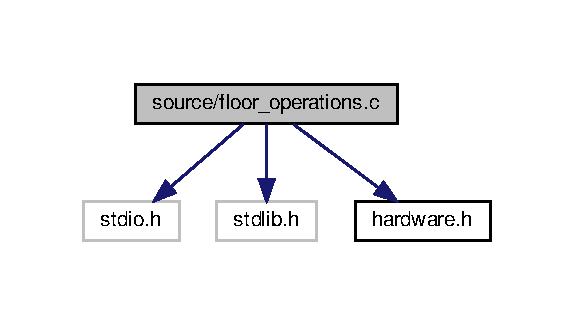
\includegraphics[width=276pt]{floor__operations_8c__incl}
\end{center}
\end{figure}
\subsection*{Functions}
\begin{DoxyCompactItemize}
\item 
\mbox{\Hypertarget{floor__operations_8c_a427ef174ce043da90cc7eed05dd926fa}\label{floor__operations_8c_a427ef174ce043da90cc7eed05dd926fa}} 
int \hyperlink{floor__operations_8c_a427ef174ce043da90cc7eed05dd926fa}{current\+\_\+floor} (int temp\+\_\+floor)
\begin{DoxyCompactList}\small\item\em return current floor \end{DoxyCompactList}\item 
\mbox{\Hypertarget{floor__operations_8c_ae66b4c87b3bec60400feed14d9a69ae0}\label{floor__operations_8c_ae66b4c87b3bec60400feed14d9a69ae0}} 
void \hyperlink{floor__operations_8c_ae66b4c87b3bec60400feed14d9a69ae0}{set\+\_\+current\+\_\+floor\+\_\+light} (int temp\+\_\+floor)
\begin{DoxyCompactList}\small\item\em turn on the lights for current floor \end{DoxyCompactList}\item 
\mbox{\Hypertarget{floor__operations_8c_a0181728ae9eaaf64fab10f8bec0504cf}\label{floor__operations_8c_a0181728ae9eaaf64fab10f8bec0504cf}} 
void \hyperlink{floor__operations_8c_a0181728ae9eaaf64fab10f8bec0504cf}{set\+\_\+and\+\_\+clear\+\_\+order\+\_\+lights} ()
\begin{DoxyCompactList}\small\item\em set and clear the order lights on the panel \end{DoxyCompactList}\item 
\mbox{\Hypertarget{floor__operations_8c_afd77151474c3e94d7c52fd75413ae3ca}\label{floor__operations_8c_afd77151474c3e94d7c52fd75413ae3ca}} 
void \hyperlink{floor__operations_8c_afd77151474c3e94d7c52fd75413ae3ca}{clear\+\_\+all\+\_\+order\+\_\+lights} ()
\begin{DoxyCompactList}\small\item\em clear all the order lights at once \end{DoxyCompactList}\item 
\mbox{\Hypertarget{floor__operations_8c_a5cd195763dabef6f126ef50f2f7cd1f5}\label{floor__operations_8c_a5cd195763dabef6f126ef50f2f7cd1f5}} 
\hyperlink{hardware_8h_a2167c399a24df296afc432bcb88228af}{Hardware\+Movement} \hyperlink{floor__operations_8c_a5cd195763dabef6f126ef50f2f7cd1f5}{choose\+\_\+init\+\_\+direction} (int U\+P\+\_\+list\mbox{[}$\,$\mbox{]}, int D\+O\+W\+N\+\_\+list\mbox{[}$\,$\mbox{]})
\begin{DoxyCompactList}\small\item\em choose movement direction when stationary \end{DoxyCompactList}\end{DoxyCompactItemize}


\subsection{Detailed Description}
Implementation of floor operation functions. 


\hypertarget{floor__operations_8h}{}\section{source/floor\+\_\+operations.h File Reference}
\label{floor__operations_8h}\index{source/floor\+\_\+operations.\+h@{source/floor\+\_\+operations.\+h}}


functions for floor operations  


This graph shows which files directly or indirectly include this file\+:\nopagebreak
\begin{figure}[H]
\begin{center}
\leavevmode
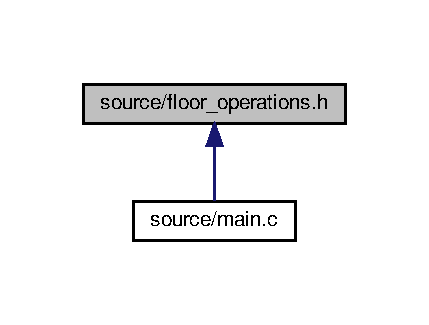
\includegraphics[width=206pt]{floor__operations_8h__dep__incl}
\end{center}
\end{figure}
\subsection*{Functions}
\begin{DoxyCompactItemize}
\item 
\mbox{\Hypertarget{floor__operations_8h_a427ef174ce043da90cc7eed05dd926fa}\label{floor__operations_8h_a427ef174ce043da90cc7eed05dd926fa}} 
int \hyperlink{floor__operations_8h_a427ef174ce043da90cc7eed05dd926fa}{current\+\_\+floor} (int temp\+\_\+floor)
\begin{DoxyCompactList}\small\item\em return current floor \end{DoxyCompactList}\item 
\mbox{\Hypertarget{floor__operations_8h_ae66b4c87b3bec60400feed14d9a69ae0}\label{floor__operations_8h_ae66b4c87b3bec60400feed14d9a69ae0}} 
void \hyperlink{floor__operations_8h_ae66b4c87b3bec60400feed14d9a69ae0}{set\+\_\+current\+\_\+floor\+\_\+light} (int temp\+\_\+floor)
\begin{DoxyCompactList}\small\item\em turn on the lights for current floor \end{DoxyCompactList}\item 
\mbox{\Hypertarget{floor__operations_8h_a0181728ae9eaaf64fab10f8bec0504cf}\label{floor__operations_8h_a0181728ae9eaaf64fab10f8bec0504cf}} 
void \hyperlink{floor__operations_8h_a0181728ae9eaaf64fab10f8bec0504cf}{set\+\_\+and\+\_\+clear\+\_\+order\+\_\+lights} ()
\begin{DoxyCompactList}\small\item\em set and clear the order lights on the panel \end{DoxyCompactList}\item 
\mbox{\Hypertarget{floor__operations_8h_afd77151474c3e94d7c52fd75413ae3ca}\label{floor__operations_8h_afd77151474c3e94d7c52fd75413ae3ca}} 
void \hyperlink{floor__operations_8h_afd77151474c3e94d7c52fd75413ae3ca}{clear\+\_\+all\+\_\+order\+\_\+lights} ()
\begin{DoxyCompactList}\small\item\em clear all the order lights at once \end{DoxyCompactList}\item 
\mbox{\Hypertarget{floor__operations_8h_a5cd195763dabef6f126ef50f2f7cd1f5}\label{floor__operations_8h_a5cd195763dabef6f126ef50f2f7cd1f5}} 
\hyperlink{hardware_8h_a2167c399a24df296afc432bcb88228af}{Hardware\+Movement} \hyperlink{floor__operations_8h_a5cd195763dabef6f126ef50f2f7cd1f5}{choose\+\_\+init\+\_\+direction} (int U\+P\+\_\+list\mbox{[}$\,$\mbox{]}, int D\+O\+W\+N\+\_\+list\mbox{[}$\,$\mbox{]})
\begin{DoxyCompactList}\small\item\em choose movement direction when stationary \end{DoxyCompactList}\end{DoxyCompactItemize}


\subsection{Detailed Description}
functions for floor operations 


\hypertarget{hardware_8h}{}\section{source/hardware.h File Reference}
\label{hardware_8h}\index{source/hardware.\+h@{source/hardware.\+h}}


Driver for the elevator hardware.  


This graph shows which files directly or indirectly include this file\+:
\nopagebreak
\begin{figure}[H]
\begin{center}
\leavevmode
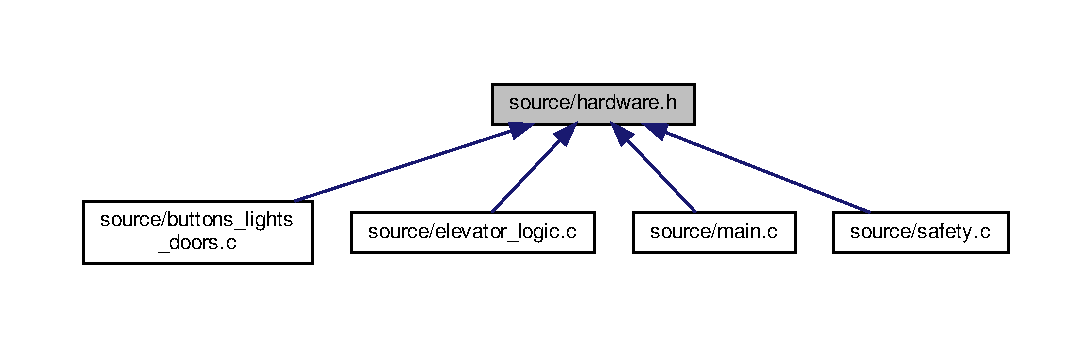
\includegraphics[width=350pt]{hardware_8h__dep__incl}
\end{center}
\end{figure}
\subsection*{Macros}
\begin{DoxyCompactItemize}
\item 
\mbox{\Hypertarget{hardware_8h_ae9e42615eade15633bd8c03b7a271a00}\label{hardware_8h_ae9e42615eade15633bd8c03b7a271a00}} 
\#define {\bfseries H\+A\+R\+D\+W\+A\+R\+E\+\_\+\+N\+U\+M\+B\+E\+R\+\_\+\+O\+F\+\_\+\+F\+L\+O\+O\+RS}~4
\end{DoxyCompactItemize}
\subsection*{Enumerations}
\begin{DoxyCompactItemize}
\item 
\mbox{\Hypertarget{hardware_8h_a2167c399a24df296afc432bcb88228af}\label{hardware_8h_a2167c399a24df296afc432bcb88228af}} 
enum \hyperlink{hardware_8h_a2167c399a24df296afc432bcb88228af}{Hardware\+Movement} \{ {\bfseries H\+A\+R\+D\+W\+A\+R\+E\+\_\+\+M\+O\+V\+E\+M\+E\+N\+T\+\_\+\+UP}, 
{\bfseries H\+A\+R\+D\+W\+A\+R\+E\+\_\+\+M\+O\+V\+E\+M\+E\+N\+T\+\_\+\+S\+T\+OP}, 
{\bfseries H\+A\+R\+D\+W\+A\+R\+E\+\_\+\+M\+O\+V\+E\+M\+E\+N\+T\+\_\+\+D\+O\+WN}
 \}\begin{DoxyCompactList}\small\item\em Movement type used in {\ttfamily hardware\+\_\+command\+\_\+movement}. \end{DoxyCompactList}
\item 
\mbox{\Hypertarget{hardware_8h_a796a8de8ce0ae769d7dbd3327a7bdbe7}\label{hardware_8h_a796a8de8ce0ae769d7dbd3327a7bdbe7}} 
enum \hyperlink{hardware_8h_a796a8de8ce0ae769d7dbd3327a7bdbe7}{Hardware\+Order} \{ {\bfseries H\+A\+R\+D\+W\+A\+R\+E\+\_\+\+O\+R\+D\+E\+R\+\_\+\+UP}, 
{\bfseries H\+A\+R\+D\+W\+A\+R\+E\+\_\+\+O\+R\+D\+E\+R\+\_\+\+I\+N\+S\+I\+DE}, 
{\bfseries H\+A\+R\+D\+W\+A\+R\+E\+\_\+\+O\+R\+D\+E\+R\+\_\+\+D\+O\+WN}
 \}\begin{DoxyCompactList}\small\item\em Order type used in {\ttfamily hardware\+\_\+read\+\_\+order} and in {\ttfamily hardware\+\_\+command\+\_\+order\+\_\+light}. \end{DoxyCompactList}
\end{DoxyCompactItemize}
\subsection*{Functions}
\begin{DoxyCompactItemize}
\item 
int \hyperlink{hardware_8h_a054b8fb8768311d46be58d6a4890d771}{hardware\+\_\+init} ()
\begin{DoxyCompactList}\small\item\em Initializes the elevator control hardware. Must be called once before other calls to the elevator hardware driver. \end{DoxyCompactList}\item 
void \hyperlink{hardware_8h_a01de081ef0510a111053c18cd31afa27}{hardware\+\_\+command\+\_\+movement} (\hyperlink{hardware_8h_a2167c399a24df296afc432bcb88228af}{Hardware\+Movement} movement)
\begin{DoxyCompactList}\small\item\em Commands the elevator to either move up or down, or commands it to halt. \end{DoxyCompactList}\item 
int \hyperlink{hardware_8h_a4a77b27c86675c00b513db3445966804}{hardware\+\_\+read\+\_\+stop\+\_\+signal} ()
\begin{DoxyCompactList}\small\item\em Polls the hardware for the current stop signal. \end{DoxyCompactList}\item 
int \hyperlink{hardware_8h_a459fe57a3ee4bc2a28e8a15b2ab14c2d}{hardware\+\_\+read\+\_\+obstruction\+\_\+signal} ()
\begin{DoxyCompactList}\small\item\em Polls the hardware for the current obstruction signal. \end{DoxyCompactList}\item 
int \hyperlink{hardware_8h_ab048489e6302bb5604aad753f2d7d501}{hardware\+\_\+read\+\_\+floor\+\_\+sensor} (int floor)
\begin{DoxyCompactList}\small\item\em Polls the floor sensor for the given {\ttfamily floor}. \end{DoxyCompactList}\item 
int \hyperlink{hardware_8h_a87917f3aa093fb46ca821a400d011ee8}{hardware\+\_\+read\+\_\+order} (int floor, \hyperlink{hardware_8h_a796a8de8ce0ae769d7dbd3327a7bdbe7}{Hardware\+Order} order\+\_\+type)
\begin{DoxyCompactList}\small\item\em Polls the hardware for the status of orders from floor {\ttfamily floor} of type {\ttfamily order\+\_\+type}. \end{DoxyCompactList}\item 
void \hyperlink{hardware_8h_a80d99ddaa8e7b58c9a88b60ea553c1b6}{hardware\+\_\+command\+\_\+door\+\_\+open} (int door\+\_\+open)
\begin{DoxyCompactList}\small\item\em Commands the hardware to open-\/ or close the elevator door. \end{DoxyCompactList}\item 
void \hyperlink{hardware_8h_a407a6ec035ba357de6aa0fbe55501d1e}{hardware\+\_\+command\+\_\+floor\+\_\+indicator\+\_\+on} (int floor)
\begin{DoxyCompactList}\small\item\em Commands the hardware to turn on the floor indicator for {\ttfamily floor}. All indicators all mutually exclusive; other indicator lights will turn off. \end{DoxyCompactList}\item 
void \hyperlink{hardware_8h_aa75b3ac17f72b25946414f48d0063a10}{hardware\+\_\+command\+\_\+stop\+\_\+light} (int on)
\begin{DoxyCompactList}\small\item\em Sets the light in the panel stop button. \end{DoxyCompactList}\item 
void \hyperlink{hardware_8h_aa9b33faa52f0ec5b614d3e7dc05be140}{hardware\+\_\+command\+\_\+order\+\_\+light} (int floor, \hyperlink{hardware_8h_a796a8de8ce0ae769d7dbd3327a7bdbe7}{Hardware\+Order} order\+\_\+type, int on)
\begin{DoxyCompactList}\small\item\em Sets the light in a button corresponding to an order of type {\ttfamily order\+\_\+type}, at floor {\ttfamily floor}. \end{DoxyCompactList}\end{DoxyCompactItemize}


\subsection{Detailed Description}
Driver for the elevator hardware. 

Neatly wraps up Martin Korsgaard\textquotesingle{}s spaghetti from 2006 ;)

Kolbjørn Austreng 

\subsection{Function Documentation}
\mbox{\Hypertarget{hardware_8h_a80d99ddaa8e7b58c9a88b60ea553c1b6}\label{hardware_8h_a80d99ddaa8e7b58c9a88b60ea553c1b6}} 
\index{hardware.\+h@{hardware.\+h}!hardware\+\_\+command\+\_\+door\+\_\+open@{hardware\+\_\+command\+\_\+door\+\_\+open}}
\index{hardware\+\_\+command\+\_\+door\+\_\+open@{hardware\+\_\+command\+\_\+door\+\_\+open}!hardware.\+h@{hardware.\+h}}
\subsubsection{\texorpdfstring{hardware\+\_\+command\+\_\+door\+\_\+open()}{hardware\_command\_door\_open()}}
{\footnotesize\ttfamily void hardware\+\_\+command\+\_\+door\+\_\+open (\begin{DoxyParamCaption}\item[{int}]{door\+\_\+open }\end{DoxyParamCaption})}



Commands the hardware to open-\/ or close the elevator door. 


\begin{DoxyParams}{Parameters}
{\em door\+\_\+open} & A truthy value (non-\/zero) to open the door; 0 to close. \\
\hline
\end{DoxyParams}
\mbox{\Hypertarget{hardware_8h_a407a6ec035ba357de6aa0fbe55501d1e}\label{hardware_8h_a407a6ec035ba357de6aa0fbe55501d1e}} 
\index{hardware.\+h@{hardware.\+h}!hardware\+\_\+command\+\_\+floor\+\_\+indicator\+\_\+on@{hardware\+\_\+command\+\_\+floor\+\_\+indicator\+\_\+on}}
\index{hardware\+\_\+command\+\_\+floor\+\_\+indicator\+\_\+on@{hardware\+\_\+command\+\_\+floor\+\_\+indicator\+\_\+on}!hardware.\+h@{hardware.\+h}}
\subsubsection{\texorpdfstring{hardware\+\_\+command\+\_\+floor\+\_\+indicator\+\_\+on()}{hardware\_command\_floor\_indicator\_on()}}
{\footnotesize\ttfamily void hardware\+\_\+command\+\_\+floor\+\_\+indicator\+\_\+on (\begin{DoxyParamCaption}\item[{int}]{floor }\end{DoxyParamCaption})}



Commands the hardware to turn on the floor indicator for {\ttfamily floor}. All indicators all mutually exclusive; other indicator lights will turn off. 


\begin{DoxyParams}{Parameters}
{\em floor} & Floor to turn on the indicator for.\\
\hline
\end{DoxyParams}
\begin{DoxyWarning}{Warning}
Owing to peculiarities in the hardware construction, there will always be one indicator active. 
\end{DoxyWarning}
\mbox{\Hypertarget{hardware_8h_a01de081ef0510a111053c18cd31afa27}\label{hardware_8h_a01de081ef0510a111053c18cd31afa27}} 
\index{hardware.\+h@{hardware.\+h}!hardware\+\_\+command\+\_\+movement@{hardware\+\_\+command\+\_\+movement}}
\index{hardware\+\_\+command\+\_\+movement@{hardware\+\_\+command\+\_\+movement}!hardware.\+h@{hardware.\+h}}
\subsubsection{\texorpdfstring{hardware\+\_\+command\+\_\+movement()}{hardware\_command\_movement()}}
{\footnotesize\ttfamily void hardware\+\_\+command\+\_\+movement (\begin{DoxyParamCaption}\item[{\hyperlink{hardware_8h_a2167c399a24df296afc432bcb88228af}{Hardware\+Movement}}]{movement }\end{DoxyParamCaption})}



Commands the elevator to either move up or down, or commands it to halt. 


\begin{DoxyParams}{Parameters}
{\em movement} & Commanded movement. \\
\hline
\end{DoxyParams}
\mbox{\Hypertarget{hardware_8h_aa9b33faa52f0ec5b614d3e7dc05be140}\label{hardware_8h_aa9b33faa52f0ec5b614d3e7dc05be140}} 
\index{hardware.\+h@{hardware.\+h}!hardware\+\_\+command\+\_\+order\+\_\+light@{hardware\+\_\+command\+\_\+order\+\_\+light}}
\index{hardware\+\_\+command\+\_\+order\+\_\+light@{hardware\+\_\+command\+\_\+order\+\_\+light}!hardware.\+h@{hardware.\+h}}
\subsubsection{\texorpdfstring{hardware\+\_\+command\+\_\+order\+\_\+light()}{hardware\_command\_order\_light()}}
{\footnotesize\ttfamily void hardware\+\_\+command\+\_\+order\+\_\+light (\begin{DoxyParamCaption}\item[{int}]{floor,  }\item[{\hyperlink{hardware_8h_a796a8de8ce0ae769d7dbd3327a7bdbe7}{Hardware\+Order}}]{order\+\_\+type,  }\item[{int}]{on }\end{DoxyParamCaption})}



Sets the light in a button corresponding to an order of type {\ttfamily order\+\_\+type}, at floor {\ttfamily floor}. 


\begin{DoxyParams}{Parameters}
{\em floor} & The floor of the order indicator. \\
\hline
{\em order\+\_\+type} & The type of order. \\
\hline
{\em on} & A truthy value (non-\/zero) to turn the light on; 0 to turn it off. \\
\hline
\end{DoxyParams}
\mbox{\Hypertarget{hardware_8h_aa75b3ac17f72b25946414f48d0063a10}\label{hardware_8h_aa75b3ac17f72b25946414f48d0063a10}} 
\index{hardware.\+h@{hardware.\+h}!hardware\+\_\+command\+\_\+stop\+\_\+light@{hardware\+\_\+command\+\_\+stop\+\_\+light}}
\index{hardware\+\_\+command\+\_\+stop\+\_\+light@{hardware\+\_\+command\+\_\+stop\+\_\+light}!hardware.\+h@{hardware.\+h}}
\subsubsection{\texorpdfstring{hardware\+\_\+command\+\_\+stop\+\_\+light()}{hardware\_command\_stop\_light()}}
{\footnotesize\ttfamily void hardware\+\_\+command\+\_\+stop\+\_\+light (\begin{DoxyParamCaption}\item[{int}]{on }\end{DoxyParamCaption})}



Sets the light in the panel stop button. 


\begin{DoxyParams}{Parameters}
{\em on} & A truthy value (non-\/zero) to turn the light on; 0 to turn it off. \\
\hline
\end{DoxyParams}
\mbox{\Hypertarget{hardware_8h_a054b8fb8768311d46be58d6a4890d771}\label{hardware_8h_a054b8fb8768311d46be58d6a4890d771}} 
\index{hardware.\+h@{hardware.\+h}!hardware\+\_\+init@{hardware\+\_\+init}}
\index{hardware\+\_\+init@{hardware\+\_\+init}!hardware.\+h@{hardware.\+h}}
\subsubsection{\texorpdfstring{hardware\+\_\+init()}{hardware\_init()}}
{\footnotesize\ttfamily int hardware\+\_\+init (\begin{DoxyParamCaption}{ }\end{DoxyParamCaption})}



Initializes the elevator control hardware. Must be called once before other calls to the elevator hardware driver. 

\begin{DoxyReturn}{Returns}
0 on success. Non-\/zero for failure. 
\end{DoxyReturn}
\mbox{\Hypertarget{hardware_8h_ab048489e6302bb5604aad753f2d7d501}\label{hardware_8h_ab048489e6302bb5604aad753f2d7d501}} 
\index{hardware.\+h@{hardware.\+h}!hardware\+\_\+read\+\_\+floor\+\_\+sensor@{hardware\+\_\+read\+\_\+floor\+\_\+sensor}}
\index{hardware\+\_\+read\+\_\+floor\+\_\+sensor@{hardware\+\_\+read\+\_\+floor\+\_\+sensor}!hardware.\+h@{hardware.\+h}}
\subsubsection{\texorpdfstring{hardware\+\_\+read\+\_\+floor\+\_\+sensor()}{hardware\_read\_floor\_sensor()}}
{\footnotesize\ttfamily int hardware\+\_\+read\+\_\+floor\+\_\+sensor (\begin{DoxyParamCaption}\item[{int}]{floor }\end{DoxyParamCaption})}



Polls the floor sensor for the given {\ttfamily floor}. 


\begin{DoxyParams}{Parameters}
{\em floor} & Inquired floor.\\
\hline
\end{DoxyParams}
\begin{DoxyReturn}{Returns}
1 if the elevator is at {\ttfamily floor}, otherwise 0; 
\end{DoxyReturn}
\mbox{\Hypertarget{hardware_8h_a459fe57a3ee4bc2a28e8a15b2ab14c2d}\label{hardware_8h_a459fe57a3ee4bc2a28e8a15b2ab14c2d}} 
\index{hardware.\+h@{hardware.\+h}!hardware\+\_\+read\+\_\+obstruction\+\_\+signal@{hardware\+\_\+read\+\_\+obstruction\+\_\+signal}}
\index{hardware\+\_\+read\+\_\+obstruction\+\_\+signal@{hardware\+\_\+read\+\_\+obstruction\+\_\+signal}!hardware.\+h@{hardware.\+h}}
\subsubsection{\texorpdfstring{hardware\+\_\+read\+\_\+obstruction\+\_\+signal()}{hardware\_read\_obstruction\_signal()}}
{\footnotesize\ttfamily int hardware\+\_\+read\+\_\+obstruction\+\_\+signal (\begin{DoxyParamCaption}{ }\end{DoxyParamCaption})}



Polls the hardware for the current obstruction signal. 

\begin{DoxyReturn}{Returns}
1 if the obstruction signal is high; 0 if it is low. 
\end{DoxyReturn}
\mbox{\Hypertarget{hardware_8h_a87917f3aa093fb46ca821a400d011ee8}\label{hardware_8h_a87917f3aa093fb46ca821a400d011ee8}} 
\index{hardware.\+h@{hardware.\+h}!hardware\+\_\+read\+\_\+order@{hardware\+\_\+read\+\_\+order}}
\index{hardware\+\_\+read\+\_\+order@{hardware\+\_\+read\+\_\+order}!hardware.\+h@{hardware.\+h}}
\subsubsection{\texorpdfstring{hardware\+\_\+read\+\_\+order()}{hardware\_read\_order()}}
{\footnotesize\ttfamily int hardware\+\_\+read\+\_\+order (\begin{DoxyParamCaption}\item[{int}]{floor,  }\item[{\hyperlink{hardware_8h_a796a8de8ce0ae769d7dbd3327a7bdbe7}{Hardware\+Order}}]{order\+\_\+type }\end{DoxyParamCaption})}



Polls the hardware for the status of orders from floor {\ttfamily floor} of type {\ttfamily order\+\_\+type}. 


\begin{DoxyParams}{Parameters}
{\em floor} & Inquired floor. \\
\hline
{\em order\+\_\+type} & \\
\hline
\end{DoxyParams}
\begin{DoxyReturn}{Returns}
1 if the combination of {\ttfamily floor} and {\ttfamily order\+\_\+type} is being requested, otherwise 0. 
\end{DoxyReturn}
\mbox{\Hypertarget{hardware_8h_a4a77b27c86675c00b513db3445966804}\label{hardware_8h_a4a77b27c86675c00b513db3445966804}} 
\index{hardware.\+h@{hardware.\+h}!hardware\+\_\+read\+\_\+stop\+\_\+signal@{hardware\+\_\+read\+\_\+stop\+\_\+signal}}
\index{hardware\+\_\+read\+\_\+stop\+\_\+signal@{hardware\+\_\+read\+\_\+stop\+\_\+signal}!hardware.\+h@{hardware.\+h}}
\subsubsection{\texorpdfstring{hardware\+\_\+read\+\_\+stop\+\_\+signal()}{hardware\_read\_stop\_signal()}}
{\footnotesize\ttfamily int hardware\+\_\+read\+\_\+stop\+\_\+signal (\begin{DoxyParamCaption}{ }\end{DoxyParamCaption})}



Polls the hardware for the current stop signal. 

\begin{DoxyReturn}{Returns}
1 if the stop signal is high; 0 if it is low. 
\end{DoxyReturn}

\hypertarget{main_8c}{}\section{source/main.c File Reference}
\label{main_8c}\index{source/main.\+c@{source/main.\+c}}


main file for running the elevator code  


{\ttfamily \#include $<$stdio.\+h$>$}\newline
{\ttfamily \#include $<$stdlib.\+h$>$}\newline
{\ttfamily \#include $<$signal.\+h$>$}\newline
{\ttfamily \#include \char`\"{}hardware.\+h\char`\"{}}\newline
{\ttfamily \#include \char`\"{}floor\+\_\+operations.\+h\char`\"{}}\newline
{\ttfamily \#include \char`\"{}button\+\_\+operations.\+h\char`\"{}}\newline
{\ttfamily \#include \char`\"{}order\+\_\+functions.\+h\char`\"{}}\newline
{\ttfamily \#include $<$time.\+h$>$}\newline
{\ttfamily \#include $<$unistd.\+h$>$}\newline
Include dependency graph for main.\+c\+:
\nopagebreak
\begin{figure}[H]
\begin{center}
\leavevmode
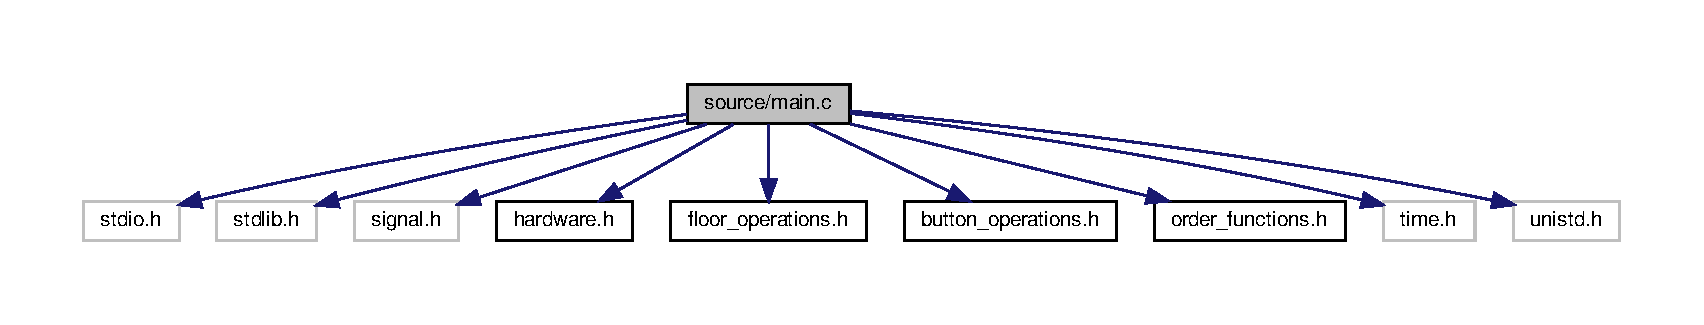
\includegraphics[width=350pt]{main_8c__incl}
\end{center}
\end{figure}
\subsection*{Functions}
\begin{DoxyCompactItemize}
\item 
int \hyperlink{main_8c_ae66f6b31b5ad750f1fe042a706a4e3d4}{main} ()
\end{DoxyCompactItemize}


\subsection{Detailed Description}
main file for running the elevator code 



\subsection{Function Documentation}
\mbox{\Hypertarget{main_8c_ae66f6b31b5ad750f1fe042a706a4e3d4}\label{main_8c_ae66f6b31b5ad750f1fe042a706a4e3d4}} 
\index{main.\+c@{main.\+c}!main@{main}}
\index{main@{main}!main.\+c@{main.\+c}}
\subsubsection{\texorpdfstring{main()}{main()}}
{\footnotesize\ttfamily int main (\begin{DoxyParamCaption}{ }\end{DoxyParamCaption})}

for(int f = 0; f $<$ H\+A\+R\+D\+W\+A\+R\+E\+\_\+\+N\+U\+M\+B\+E\+R\+\_\+\+O\+F\+\_\+\+F\+L\+O\+O\+RS; f++)\{ if(hardware\+\_\+read\+\_\+order(f, H\+A\+R\+D\+W\+A\+R\+E\+\_\+\+O\+R\+D\+E\+R\+\_\+\+I\+N\+S\+I\+D\+E))\{ hardware\+\_\+command\+\_\+floor\+\_\+indicator\+\_\+on(f); \} \}

Definition at line 16 of file main.\+c.


\hypertarget{order__functions_8c}{}\section{source/order\+\_\+functions.c File Reference}
\label{order__functions_8c}\index{source/order\+\_\+functions.\+c@{source/order\+\_\+functions.\+c}}


implementation of order functions  


{\ttfamily \#include $<$stdio.\+h$>$}\newline
{\ttfamily \#include $<$stdlib.\+h$>$}\newline
{\ttfamily \#include \char`\"{}hardware.\+h\char`\"{}}\newline
Include dependency graph for order\+\_\+functions.\+c\+:\nopagebreak
\begin{figure}[H]
\begin{center}
\leavevmode
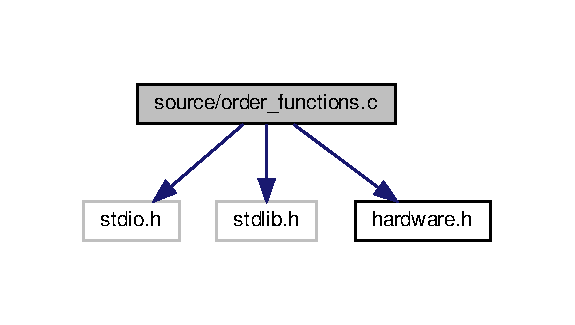
\includegraphics[width=276pt]{order__functions_8c__incl}
\end{center}
\end{figure}
\subsection*{Functions}
\begin{DoxyCompactItemize}
\item 
\mbox{\Hypertarget{order__functions_8c_afe21df0455a7cb03dbd9c9294697704e}\label{order__functions_8c_afe21df0455a7cb03dbd9c9294697704e}} 
void \hyperlink{order__functions_8c_afe21df0455a7cb03dbd9c9294697704e}{set\+\_\+\+U\+P\+\_\+list} (int U\+P\+\_\+list\mbox{[}$\,$\mbox{]})
\begin{DoxyCompactList}\small\item\em set list of orders going UP \end{DoxyCompactList}\item 
\mbox{\Hypertarget{order__functions_8c_aebbe53837d376172d3029098cbf0e005}\label{order__functions_8c_aebbe53837d376172d3029098cbf0e005}} 
void \hyperlink{order__functions_8c_aebbe53837d376172d3029098cbf0e005}{set\+\_\+\+D\+O\+W\+N\+\_\+list} (int D\+O\+W\+N\+\_\+list\mbox{[}$\,$\mbox{]})
\begin{DoxyCompactList}\small\item\em set list of orders going D\+O\+WN \end{DoxyCompactList}\end{DoxyCompactItemize}


\subsection{Detailed Description}
implementation of order functions 


\hypertarget{order__functions_8h}{}\section{source/order\+\_\+functions.h File Reference}
\label{order__functions_8h}\index{source/order\+\_\+functions.\+h@{source/order\+\_\+functions.\+h}}


functions for orders  


This graph shows which files directly or indirectly include this file\+:
\nopagebreak
\begin{figure}[H]
\begin{center}
\leavevmode
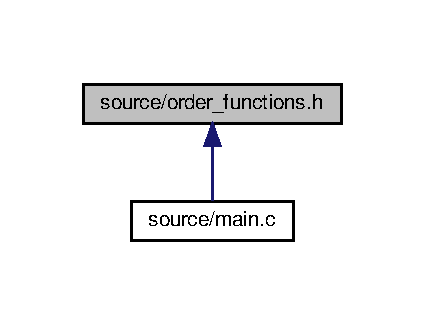
\includegraphics[width=204pt]{order__functions_8h__dep__incl}
\end{center}
\end{figure}
\subsection*{Functions}
\begin{DoxyCompactItemize}
\item 
\mbox{\Hypertarget{order__functions_8h_afe21df0455a7cb03dbd9c9294697704e}\label{order__functions_8h_afe21df0455a7cb03dbd9c9294697704e}} 
void \hyperlink{order__functions_8h_afe21df0455a7cb03dbd9c9294697704e}{set\+\_\+\+U\+P\+\_\+list} (int U\+P\+\_\+list\mbox{[}$\,$\mbox{]})
\begin{DoxyCompactList}\small\item\em set list of orders going UP \end{DoxyCompactList}\item 
\mbox{\Hypertarget{order__functions_8h_aebbe53837d376172d3029098cbf0e005}\label{order__functions_8h_aebbe53837d376172d3029098cbf0e005}} 
void \hyperlink{order__functions_8h_aebbe53837d376172d3029098cbf0e005}{set\+\_\+\+D\+O\+W\+N\+\_\+list} (int D\+O\+W\+N\+\_\+list\mbox{[}$\,$\mbox{]})
\begin{DoxyCompactList}\small\item\em set list of orders going D\+O\+WN \end{DoxyCompactList}\item 
\mbox{\Hypertarget{order__functions_8h_a7138e071e2242ce623c49f435a83cc12}\label{order__functions_8h_a7138e071e2242ce623c49f435a83cc12}} 
void {\bfseries handle\+\_\+inside\+\_\+order} (int \hyperlink{floor__operations_8h_a427ef174ce043da90cc7eed05dd926fa}{current\+\_\+floor}, int U\+P\+\_\+list\mbox{[}$\,$\mbox{]}, int D\+O\+W\+N\+\_\+list\mbox{[}$\,$\mbox{]})
\end{DoxyCompactItemize}


\subsection{Detailed Description}
functions for orders 


%--- End generated contents ---

% Index
\backmatter
\newpage
\phantomsection
\clearemptydoublepage
\addcontentsline{toc}{chapter}{Index}
\printindex

\end{document}
